
\documentclass[12pt]{article}
\usepackage[T1]{fontenc}
\usepackage{hyperref}
\usepackage{amsmath}
\usepackage{graphicx}
\usepackage{tikz, mhchem}
\usepackage{mathtools}

\setcounter{figure}{0}

\title{Free Amino Acids in Human Milk: Time and Infant Gender}
\author{Federico J. Zertuche}
\date{\today}

\begin{document}
\maketitle

\begin{abstract}
This report is about comparing our results with those in the litterature, specifically those found here:

\begin{center}
  \href{https://www.mdpi.com/2072-6643/10/9/1233}{https://www.mdpi.com/2072-6643/10/9/1233}
\end{center}

It is divided into $3$ parts:

The first part is about understanding the data. I try to describe and motivate the models, significant results and thier relationship with existing literature and medical knowledge.

The second part is about what should you be looking forward to in future experiments. Here, I take the models seriously and device possible predictions that are compatible with current knowledge.

The third part is about missing data. I mention what I did with the missing patients.

\end{abstract}

\part{Three Objectives, Three Models}

I am interested in answering $3$ questions:

\begin{enumerate}
  \item Do amino acid levels change over time?
  \item Are these levels different in the milk for boys and girls?
  \item If the concentration changes over time, is it different for boys and girls?
\end{enumerate}

I use $3$ regression models to summarize the effects for each one of the questions. The answers are given as coefficients with confidence intervlas.

Before analyzing the results let me introduce some notation.

I will write $AA$ for the concentration level of a particular amino acid. The data contains the concentration of several amino acids. In general, I will study them individually. I use the essential and non essential classification since I am interested in the difference between nourishment and body production.

The measurements were taken at weeks $1, 2, 8$ and $16$ so the variable corresponding to time is called $week$. This is not a categorical variable.

I note the infant genders $boy$ and $girl$ and the variable will be called $sex$.

There is an additional variable called $group$ that tells us if the mother was a $teen$ or an $adult$ when she gave birth.

\section{Do AA levels change over time?}

Here the model used is:

\begin{equation} \label{eq:model1}
  AA = \alpha_0 + \alpha_1 \ week + \alpha_{id}
\end{equation}

Each coefficient is the summary of an effect.

The first, $\alpha_0$, is the concentration at week $0$, I will not talk about this coefficint. The second one has units $concentration/time$, it is the main focus in this part of the analysis.

The last one represents a random effect that is different for each one of the participats, think about it as all the patients differences you didn't control for during data collection process.


\begin{figure}[ht]
  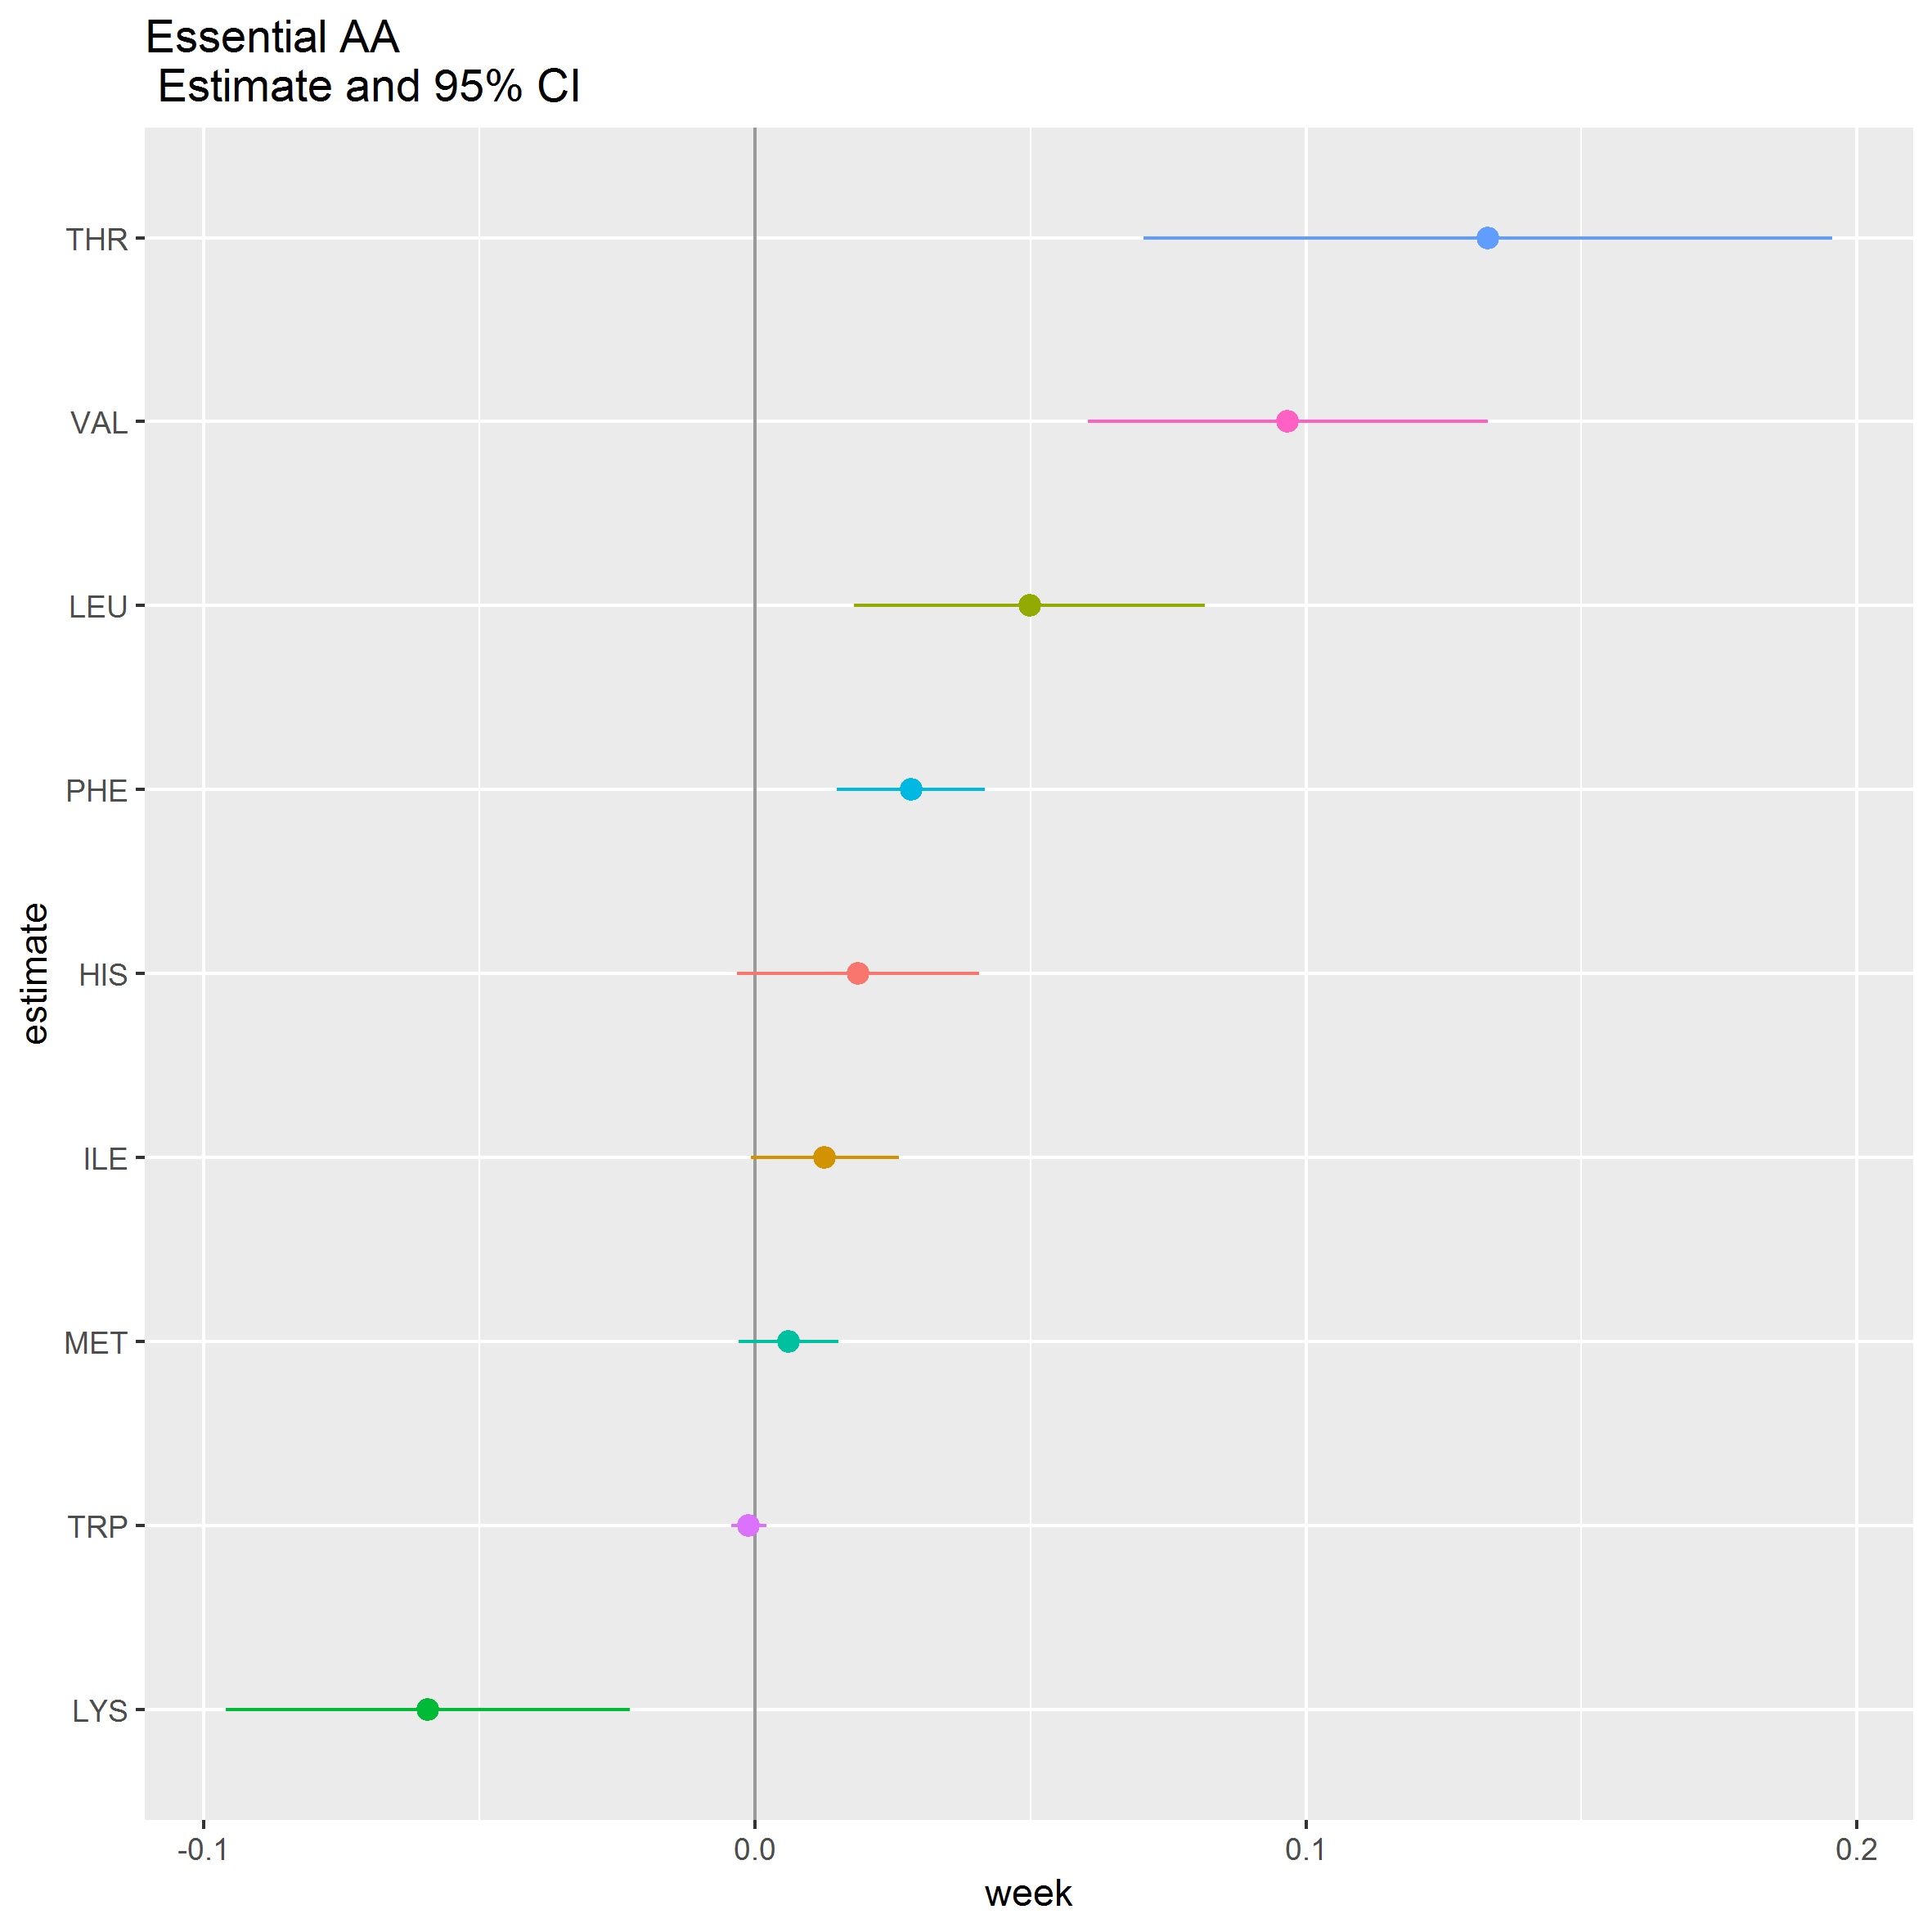
\includegraphics[width= \textwidth]{../week/EAA_W_coeff.png}
  \caption{Week coefficients of model (\ref{eq:model1}) for essential amino acids.}
  \label{fig:EAA_W_coeff}
\end{figure}

The list of amino acids with significant effects (figure \ref{fig:EAA_W_coeff}) over time is: THR, VAL, LUE, PHE. As you can see in figure (\ref{fig:EAA_simple}), in all of these amino acids, there a general trend. The coefficients are meant to capture this. 

\begin{figure}[ht]
  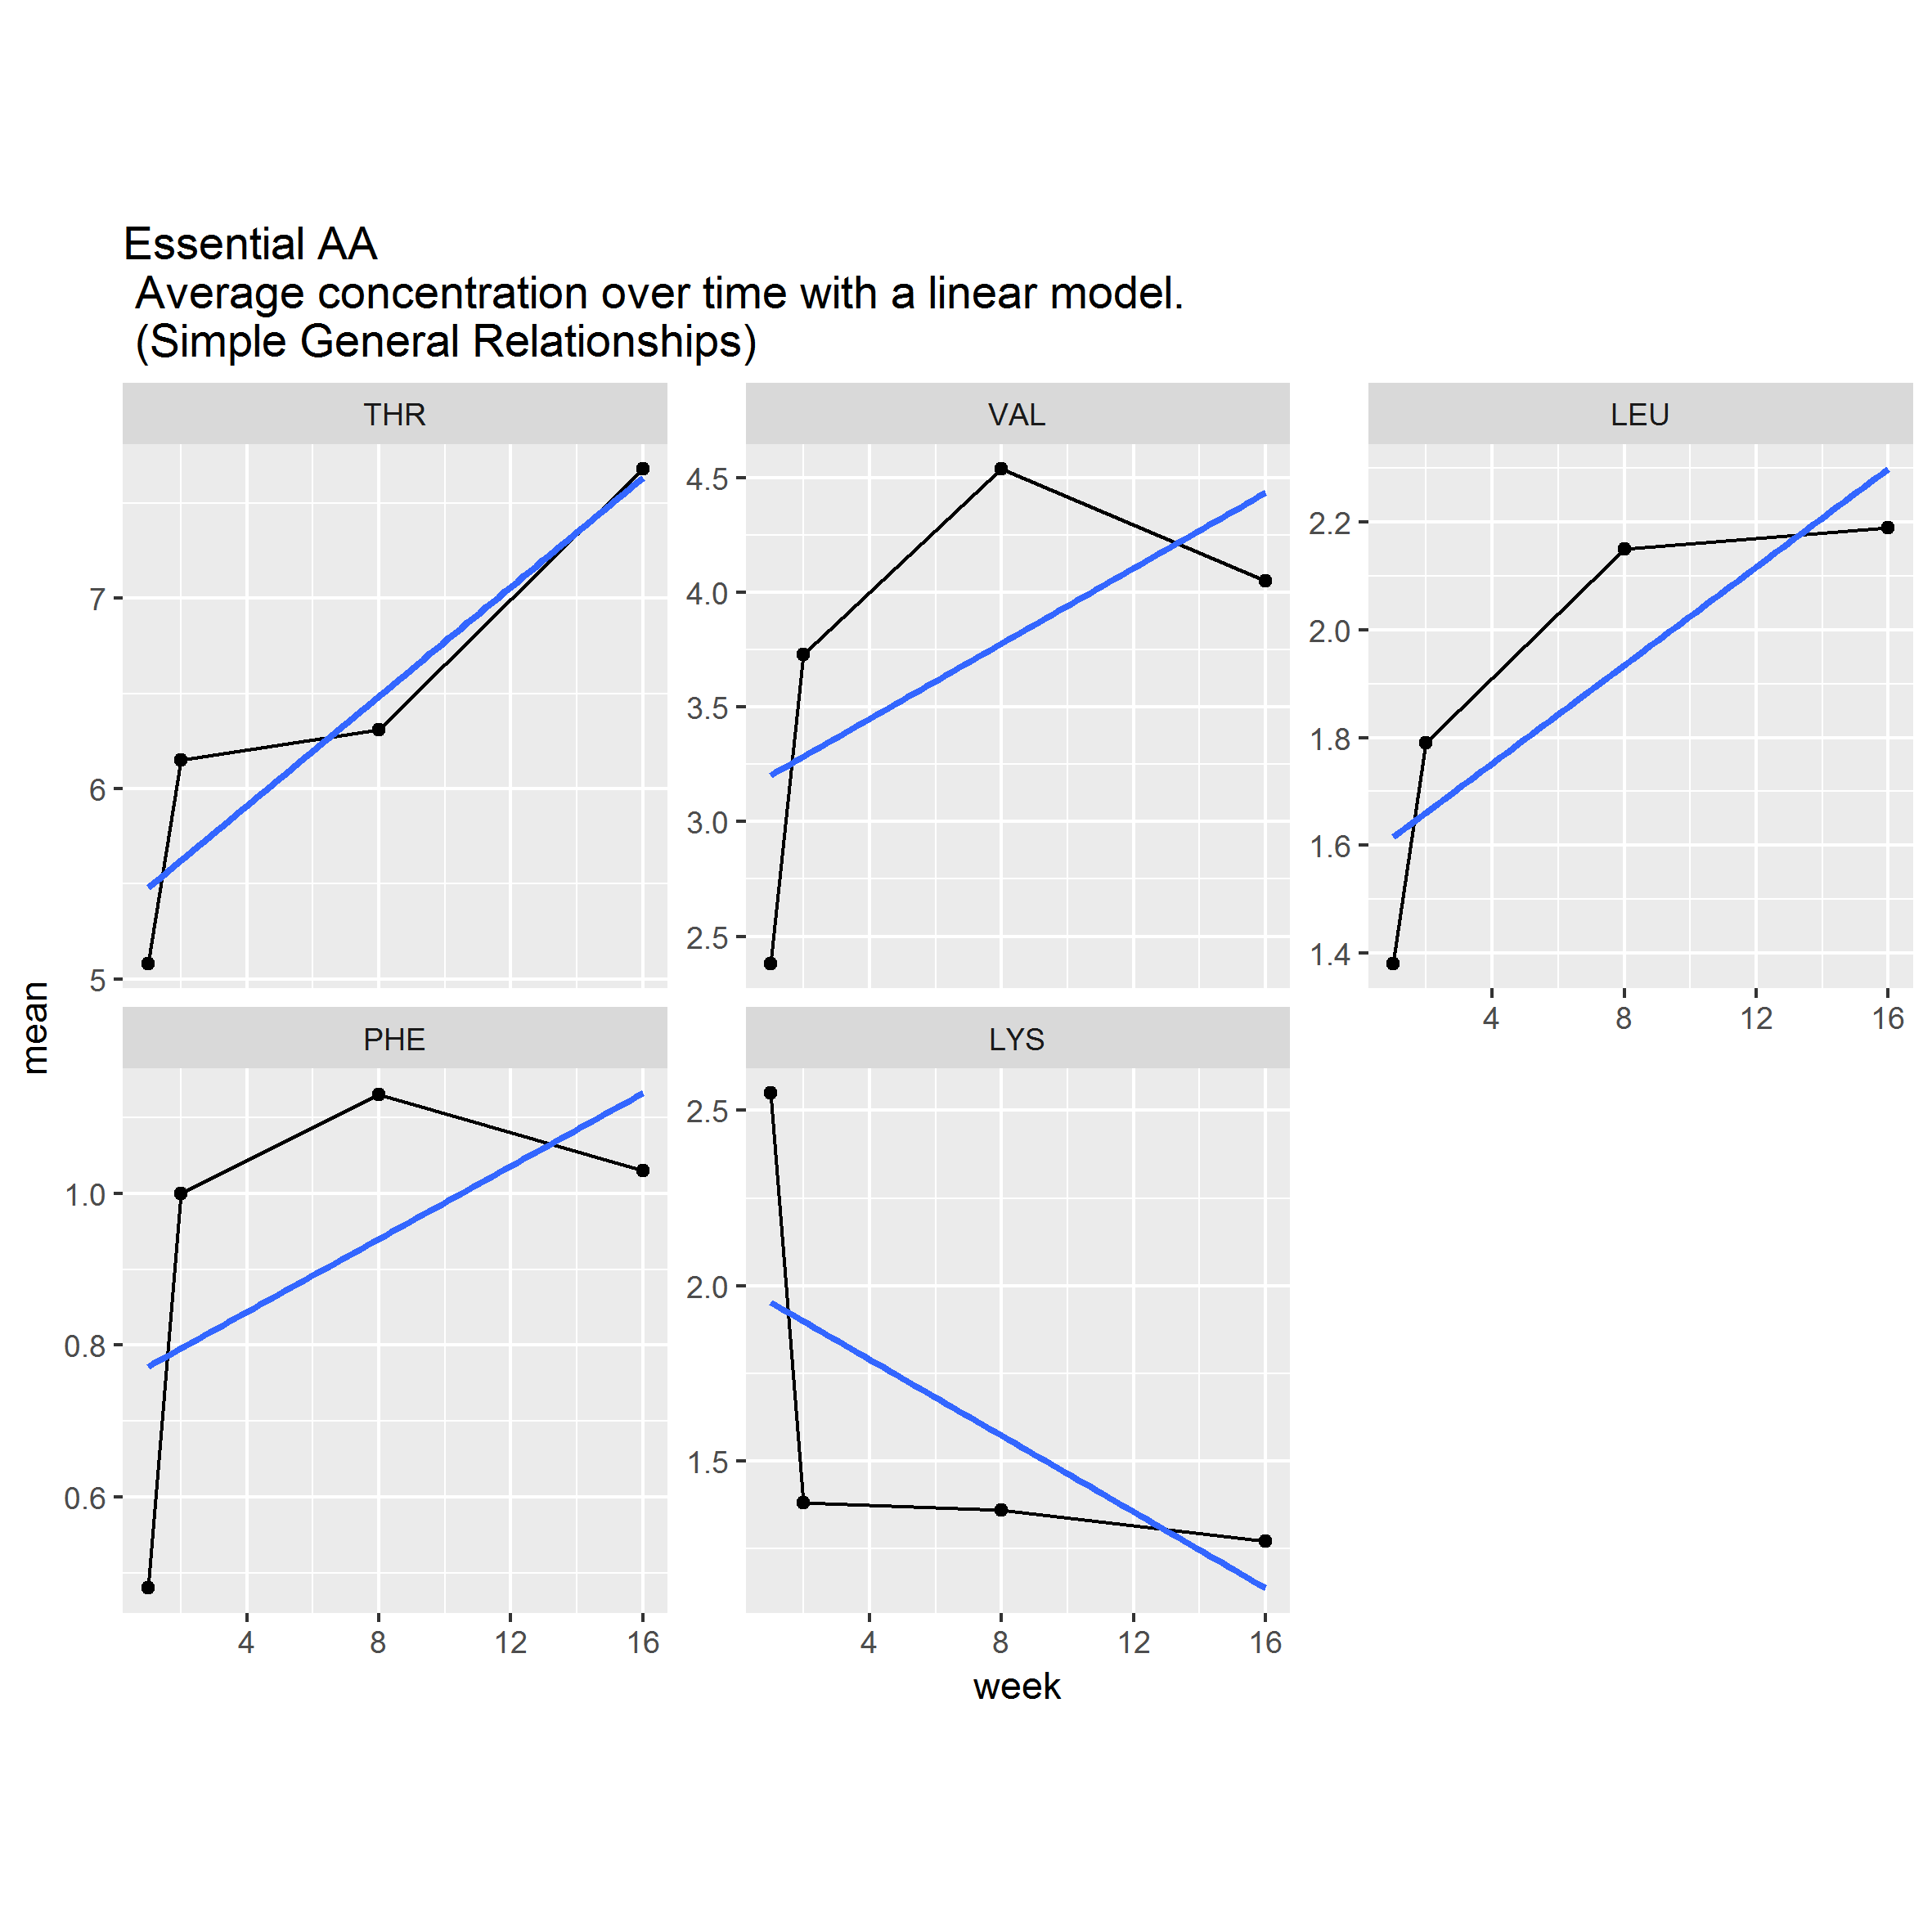
\includegraphics[width= \textwidth]{../week/EAA_simple.png}
  \caption{Mean concentration per week with a linear regression line in blue. Amino acids with significan week effects.}
  \label{fig:EAA_simple}
\end{figure}


Four amino acids have a non significant effect: HIS, ILE, MET and TRP.






% \begin{figure}[ht]\label{fig:NEAA_W_coeff}
%   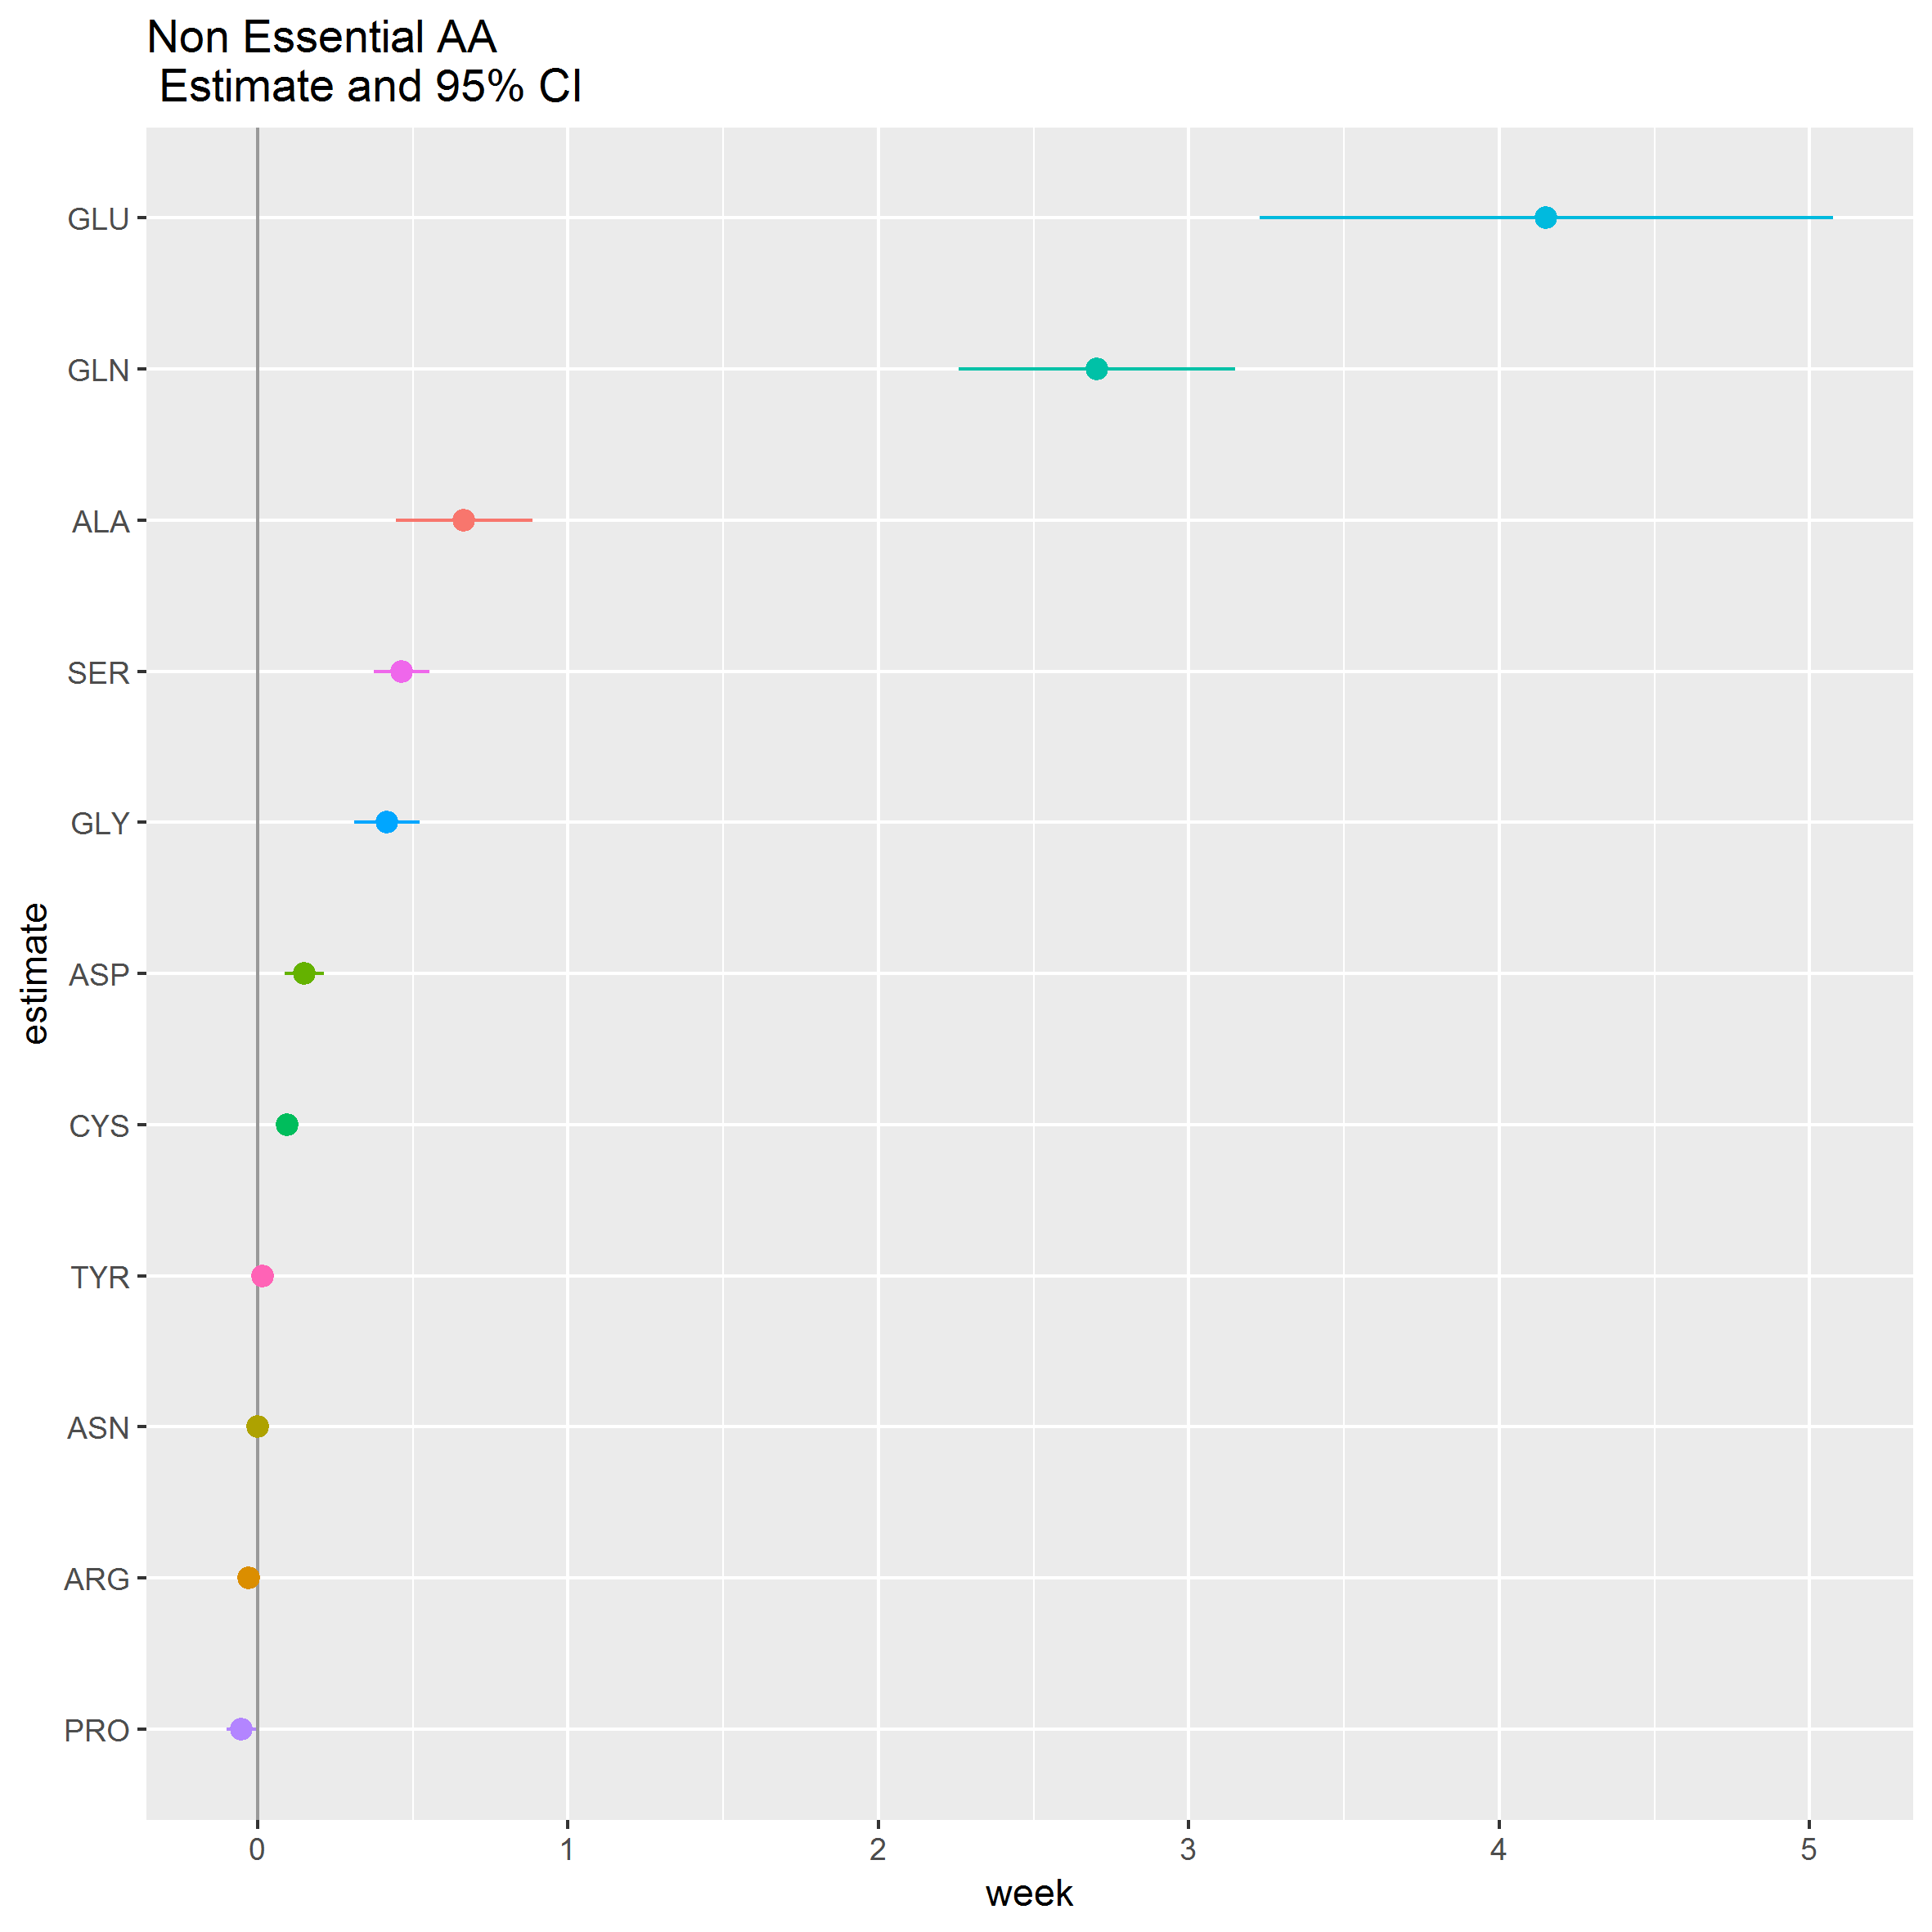
\includegraphics[width= \textwidth]{../week/NEAA_W_coeff.png}
%   \caption{Week coefficients of model (\ref{eq:model1}) for NON essential amino acids.}
% \end{figure}
%
%
% \begin{figure}[ht]\label{fig:NEAA_W_coeff_detail}
%   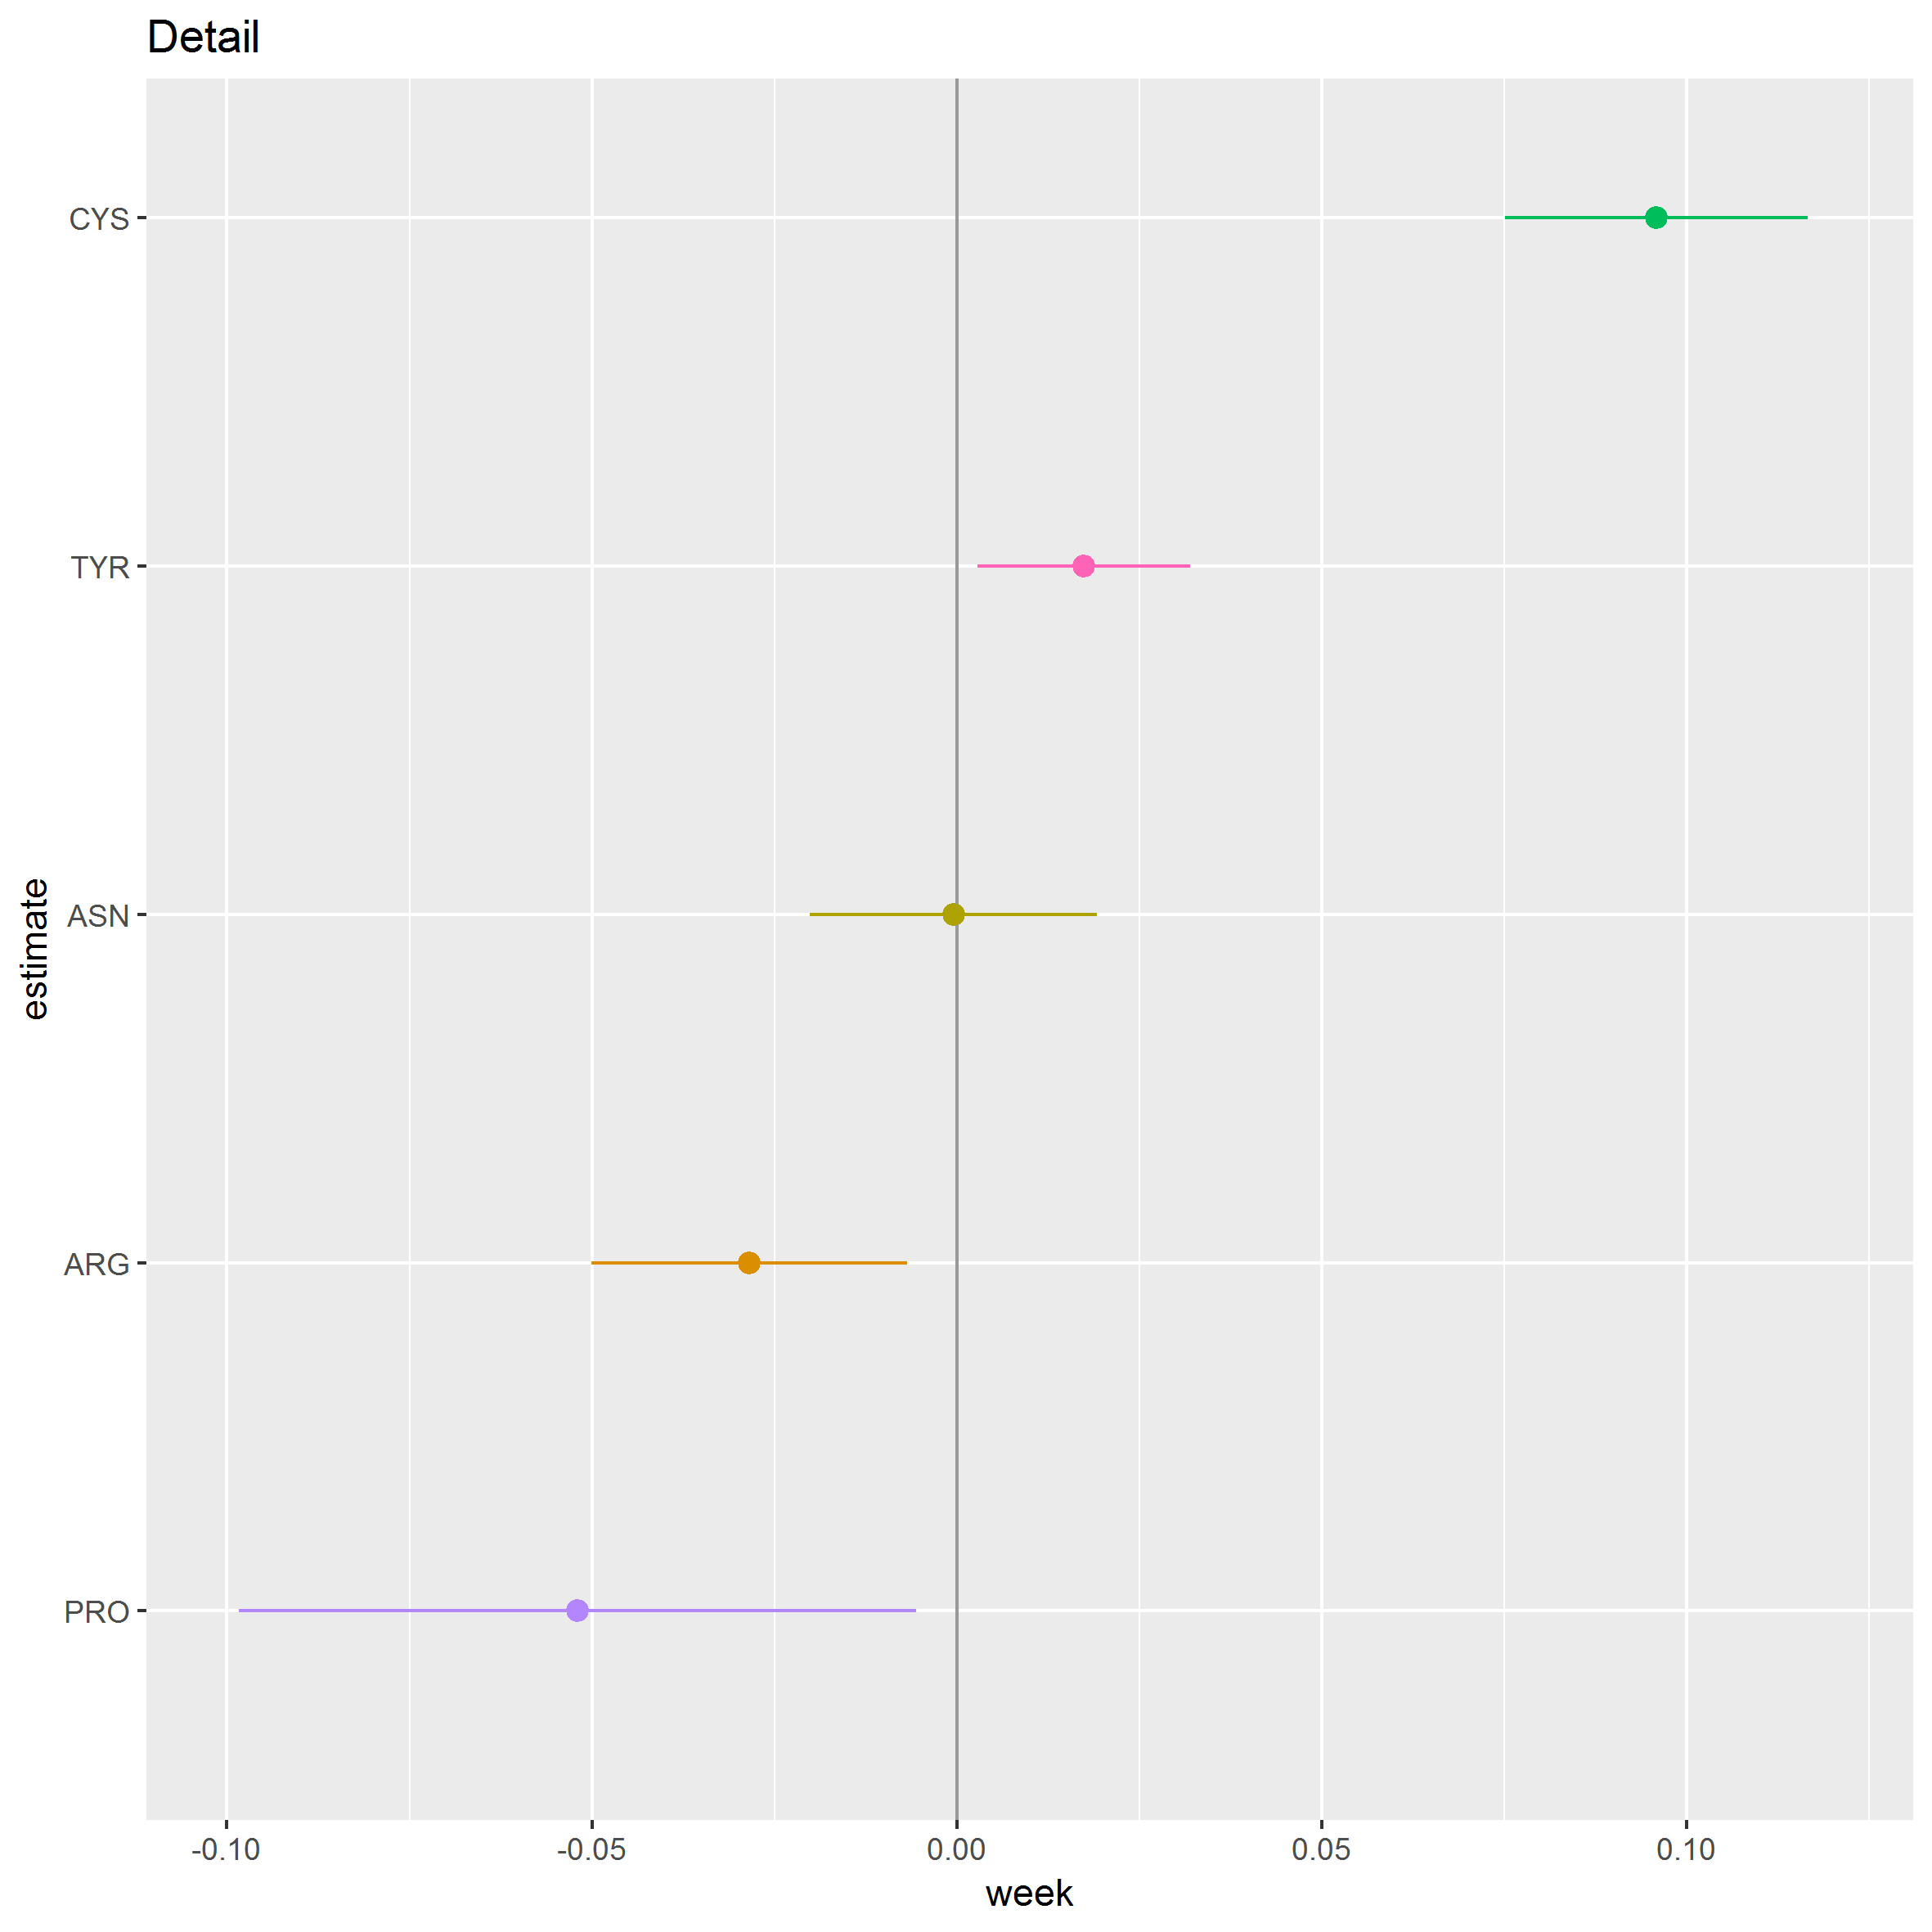
\includegraphics[width= \textwidth]{../week/NEAA_W_coeff_detail.png}
%   \caption{Detail of the last week coefficients of model (\ref{eq:model1}) for NON essential amino acids.}
% \end{figure}

%\bibliographystyle{plain}
%\bibliography{thebibliography}

%\begin{thebibliography}{1}

%\bibitem{python} Python Software Foundation. Python Language Reference, version 3.6 Available at http://www.python.org.

%\bibitem{COBRApy} COBRApy: COnstraints-Based Reconstruction and Analysis for Python,
%Ali Ebrahim, Joshua A. Lerman, Bernhard O. Palsson, and Daniel R. Hyduke,
%BMC Systems Biology, 2013, 7:74.

%\end{thebibliography}

\end{document}
This is never printed
